\documentclass[aspectratio=169]{beamer}
\usepackage{will_handley_beamer}
\usepackage{title_page}

% Commands
% --------
% - \arxiv{arxiv number}
% - \cols{width}{lh column}{rh column}
% -  \begin{fig(left|right)}[fractional width (e.g 0.6) ]{name of image}
%        content of other column
%    \end{fig(left|right)}

% Talk details
% ------------
\title{Gradients and Nested Sampling}
\subtitle{The present state of the art}
\date{7\textsuperscript{th} Jule 2023}

\begin{document}

\begin{frame}
    \titlepage
\end{frame}

\begin{frame}
    stan
    blackjax
    pyjax

    PyMC
    
    Probabilistic Programming

    PPX

    NS nodeterminism

    MAP
    
    HMC

    VI

    Laplace approximation

    density of states

    volume estimation

    roofit

    emcee

    Number of parameters
\end{frame}

\begin{frame}
    \frametitle{What is nested sampling}
    
    Buchner review \arxiv{2101.09675}

    Nature reviews primer \arxiv{2205.15570}

\end{frame}

\begin{frame}
    \frametitle{Implementations of nested sampling}
\end{frame}


\begin{frame}
    \frametitle{Using the Likelihood as part of a normal HMC}
    \begin{itemize}
        \item Nested sampling requires you to sample from the truncated \emph{prior}, not the likelihood
        \item Other than at the boundaries, it is not obvious how to use a likelihood gradient to navigate the prior.
        \item In addition, since nested sampling begins in the tails, proceeding through the typical set and onto the peak, the normalisation of the gradient is normally not very useful.
    \end{itemize}
\end{frame}

\begin{frame}
    \frametitle{Constrained Hamiltonian Monte Carlo~\arxiv{1005.0157}}
    \framesubtitle{aka: Gailean nested sampling~\arxiv{1312.5638}; Reflective slice sampling~\oldarxiv{physics/0009028}}

    \begin{columns}
        \column{0.5\textwidth}
        \begin{itemize}
            \item The primary way to sample from ``Tabletop'' distributions is with reflection:
                \begin{itemize}
                    \item Define start $x_0$, velocity $v$,
                    \item Update $x_{i+1} = x_i + v \Delta t$
                    \item When you reach the edge, reflect using $\hat{n}$:
                        $ v \to v - 2 (v\cdot \hat{n}) \hat{n}$
                    \item $n$ can be taken to be $\nabla \log P$
                \end{itemize}
            \item In practice since don't know the exact boundary, care needs to be taken to generate unbiased samples 
                \begin{itemize}
                    \item e.g. by reflecting whenever one is outside, not just once to get us back in.
                \end{itemize}
            \item Radford Neal~\oldarxiv{physics/0009028} section 7 is best reference for this.
        \end{itemize}
        
        \column{0.5\textwidth}
        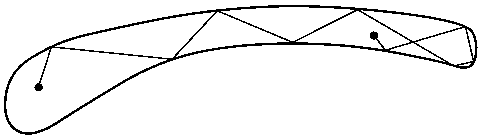
\includegraphics[width=\textwidth]{figures/reflect}
        \vspace{1em}

        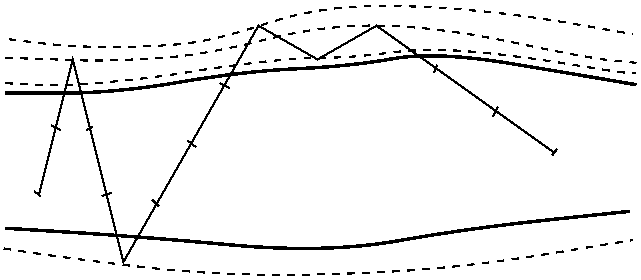
\includegraphics[width=\textwidth]{figures/bounce}
    \end{columns}

\end{frame}

\begin{frame}
    \frametitle{Historical attempts}
    \begin{itemize}
        \item Betancourt: Hamiltonian constrained nested sampling~\arxiv{1005.0157}
        \item Feroz: Galilean Nested Sampling~\arxiv{1312.5638}
        \item Incorporated into \texttt{dynesty}~\arxiv{1904.02180}
        \item Demonic nested sampling Habeck~\doi{10.1063/1.4905971} -- uses thermodynamic analogy to soften the hard boundary with a Maxwell daemon.
        \item Baldock \arxiv{1710.11085} -- Total Enthalpy HMC, incoporating momenta in a more HMC like way, but specialised to materials science
    \end{itemize}
\end{frame}

\section{Possible future avenues}
\subsection{Mass matrix rescaling}
\subsection{Posterior repartitioning}

\begin{frame}
    \frametitle{<+Frame title+>}
    <+Content+>
\end{frame}

\end{document}
